\documentclass[tikz,border=10pt]{standalone}
\usepackage{tikz}
\usetikzlibrary{calc}
\begin{document}
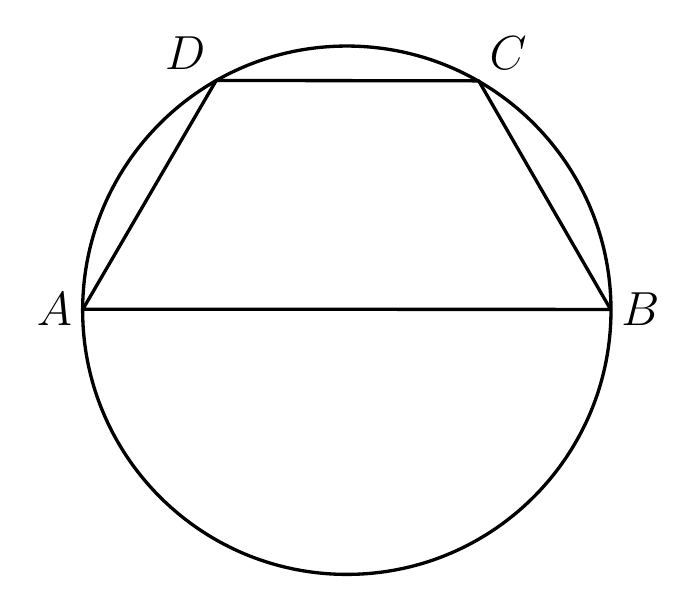
\begin{tikzpicture}[line join=round, line width=1.2pt]
  % Vertices from pixel coords: x=(px-224.29)*s, y=(201.88-py)*s, s=0.021333
  \coordinate (O) at (0,0);
  \coordinate (A) at (-3.352,0.013);
  \coordinate (B) at (3.350,0.010);
  \coordinate (C) at (1.675,2.913);
  \coordinate (D) at (-1.659,2.918);

  % Circle, radius 157.28 px = 3.355 units
  \draw (O) circle (3.355);

  % Trapezoid ABCD (solid)
  \draw (A) -- (B) -- (C) -- (D) -- cycle;

  % Labels
  \node[left] at (A) {\fontsize{17}{20.4}\selectfont $A$};
  \node[right] at (B) {\fontsize{17}{20.4}\selectfont $B$};
  \node[above right] at (C) {\fontsize{17}{20.4}\selectfont $C$};
  \node[above left] at (D) {\fontsize{17}{20.4}\selectfont $D$};
\end{tikzpicture}
\end{document}